\documentclass[portrait]{article}
\usepackage{lmodern}
\usepackage{amssymb,amsmath}
\usepackage{ifxetex,ifluatex}
\usepackage{fixltx2e} % provides \textsubscript
\ifnum 0\ifxetex 1\fi\ifluatex 1\fi=0 % if pdftex
  \usepackage[T1]{fontenc}
  \usepackage[utf8]{inputenc}
\else % if luatex or xelatex
  \ifxetex
    \usepackage{mathspec}
  \else
    \usepackage{fontspec}
  \fi
  \defaultfontfeatures{Ligatures=TeX,Scale=MatchLowercase}
\fi
% use upquote if available, for straight quotes in verbatim environments
\IfFileExists{upquote.sty}{\usepackage{upquote}}{}
% use microtype if available
\IfFileExists{microtype.sty}{%
\usepackage[]{microtype}
\UseMicrotypeSet[protrusion]{basicmath} % disable protrusion for tt fonts
}{}
\PassOptionsToPackage{hyphens}{url} % url is loaded by hyperref
\usepackage[unicode=true]{hyperref}
\hypersetup{
            pdftitle={Using RMarkdown for reproducible and neat documents},
            pdfborder={0 0 0},
            breaklinks=true}
\urlstyle{same}  % don't use monospace font for urls
\usepackage{color}
\usepackage{fancyvrb}
\newcommand{\VerbBar}{|}
\newcommand{\VERB}{\Verb[commandchars=\\\{\}]}
\DefineVerbatimEnvironment{Highlighting}{Verbatim}{commandchars=\\\{\}}
% Add ',fontsize=\small' for more characters per line
\usepackage{framed}
\definecolor{shadecolor}{RGB}{248,248,248}
\newenvironment{Shaded}{\begin{snugshade}}{\end{snugshade}}
\newcommand{\KeywordTok}[1]{\textcolor[rgb]{0.13,0.29,0.53}{\textbf{#1}}}
\newcommand{\DataTypeTok}[1]{\textcolor[rgb]{0.13,0.29,0.53}{#1}}
\newcommand{\DecValTok}[1]{\textcolor[rgb]{0.00,0.00,0.81}{#1}}
\newcommand{\BaseNTok}[1]{\textcolor[rgb]{0.00,0.00,0.81}{#1}}
\newcommand{\FloatTok}[1]{\textcolor[rgb]{0.00,0.00,0.81}{#1}}
\newcommand{\ConstantTok}[1]{\textcolor[rgb]{0.00,0.00,0.00}{#1}}
\newcommand{\CharTok}[1]{\textcolor[rgb]{0.31,0.60,0.02}{#1}}
\newcommand{\SpecialCharTok}[1]{\textcolor[rgb]{0.00,0.00,0.00}{#1}}
\newcommand{\StringTok}[1]{\textcolor[rgb]{0.31,0.60,0.02}{#1}}
\newcommand{\VerbatimStringTok}[1]{\textcolor[rgb]{0.31,0.60,0.02}{#1}}
\newcommand{\SpecialStringTok}[1]{\textcolor[rgb]{0.31,0.60,0.02}{#1}}
\newcommand{\ImportTok}[1]{#1}
\newcommand{\CommentTok}[1]{\textcolor[rgb]{0.56,0.35,0.01}{\textit{#1}}}
\newcommand{\DocumentationTok}[1]{\textcolor[rgb]{0.56,0.35,0.01}{\textbf{\textit{#1}}}}
\newcommand{\AnnotationTok}[1]{\textcolor[rgb]{0.56,0.35,0.01}{\textbf{\textit{#1}}}}
\newcommand{\CommentVarTok}[1]{\textcolor[rgb]{0.56,0.35,0.01}{\textbf{\textit{#1}}}}
\newcommand{\OtherTok}[1]{\textcolor[rgb]{0.56,0.35,0.01}{#1}}
\newcommand{\FunctionTok}[1]{\textcolor[rgb]{0.00,0.00,0.00}{#1}}
\newcommand{\VariableTok}[1]{\textcolor[rgb]{0.00,0.00,0.00}{#1}}
\newcommand{\ControlFlowTok}[1]{\textcolor[rgb]{0.13,0.29,0.53}{\textbf{#1}}}
\newcommand{\OperatorTok}[1]{\textcolor[rgb]{0.81,0.36,0.00}{\textbf{#1}}}
\newcommand{\BuiltInTok}[1]{#1}
\newcommand{\ExtensionTok}[1]{#1}
\newcommand{\PreprocessorTok}[1]{\textcolor[rgb]{0.56,0.35,0.01}{\textit{#1}}}
\newcommand{\AttributeTok}[1]{\textcolor[rgb]{0.77,0.63,0.00}{#1}}
\newcommand{\RegionMarkerTok}[1]{#1}
\newcommand{\InformationTok}[1]{\textcolor[rgb]{0.56,0.35,0.01}{\textbf{\textit{#1}}}}
\newcommand{\WarningTok}[1]{\textcolor[rgb]{0.56,0.35,0.01}{\textbf{\textit{#1}}}}
\newcommand{\AlertTok}[1]{\textcolor[rgb]{0.94,0.16,0.16}{#1}}
\newcommand{\ErrorTok}[1]{\textcolor[rgb]{0.64,0.00,0.00}{\textbf{#1}}}
\newcommand{\NormalTok}[1]{#1}
\usepackage{longtable,booktabs}
% Fix footnotes in tables (requires footnote package)
\IfFileExists{footnote.sty}{\usepackage{footnote}\makesavenoteenv{long table}}{}
\usepackage{graphicx,grffile}
\makeatletter
\def\maxwidth{\ifdim\Gin@nat@width>\linewidth\linewidth\else\Gin@nat@width\fi}
\def\maxheight{\ifdim\Gin@nat@height>\textheight\textheight\else\Gin@nat@height\fi}
\makeatother
% Scale images if necessary, so that they will not overflow the page
% margins by default, and it is still possible to overwrite the defaults
% using explicit options in \includegraphics[width, height, ...]{}
\setkeys{Gin}{width=\maxwidth,height=\maxheight,keepaspectratio}
\IfFileExists{parskip.sty}{%
\usepackage{parskip}
}{% else
\setlength{\parindent}{0pt}
\setlength{\parskip}{6pt plus 2pt minus 1pt}
}
\setlength{\emergencystretch}{3em}  % prevent overfull lines
\providecommand{\tightlist}{%
  \setlength{\itemsep}{0pt}\setlength{\parskip}{0pt}}
\setcounter{secnumdepth}{0}
% Redefines (sub)paragraphs to behave more like sections
\ifx\paragraph\undefined\else
\let\oldparagraph\paragraph
\renewcommand{\paragraph}[1]{\oldparagraph{#1}\mbox{}}
\fi
\ifx\subparagraph\undefined\else
\let\oldsubparagraph\subparagraph
\renewcommand{\subparagraph}[1]{\oldsubparagraph{#1}\mbox{}}
\fi

% set default figure placement to htbp
\makeatletter
\def\fps@figure{htbp}
\makeatother


\title{Using RMarkdown for reproducible and neat documents}
\author{Your name here\\[2\baselineskip]Your affiliation here}
\date{}

\begin{document}
\maketitle

{
\setcounter{tocdepth}{4}
\tableofcontents
}
\newpage   

Date: 2019-10-22\\
R version: 3.5.0\\
*Corresponding author: your email here

\newpage    

\section{Overview}\label{overview}

This document showcases how to create and use \texttt{RMarkdown}
documents.

You can write in \textbf{bold} and \emph{italicised} text (in \emph{two}
different \textbf{ways}).

You can write in-line \texttt{code} if you want to differentiate between
when you are typing normally or highlighting \texttt{model\ parameters},
for example.

Equations like this \(t' = \gamma(t - vx/c^{2})\), to appear within text
lines.

Create links to your \href{https://github.com/darwinanddavis}{website}.

Make footnotes\footnote{Here is the footnote you created earlier,
  automatically formatted}.

\section{\texorpdfstring{You can easily create headings. This is the
same font size as the `Overview'
above}{You can easily create headings. This is the same font size as the Overview above}}\label{you-can-easily-create-headings.-this-is-the-same-font-size-as-the-overview-above}

\subsection{Then move down in font
size}\label{then-move-down-in-font-size}

\subsubsection{Like this subheading}\label{like-this-subheading}

\paragraph{And this fourth order
heading}\label{and-this-fourth-order-heading}

Insert line breaks between text like this

Insert a horizontal line break using five asterisks (`*****')

\begin{center}\rule{0.5\linewidth}{\linethickness}\end{center}

(There is also a page break here. Best seen in PDF. Check the raw Rmd
file to see the code)

The raw Rmd file also has the code for inserting user comments,

\newpage    

\subsection{Define equations}\label{define-equations}

Accordingly, we write the eigenfunction of a spinless particle as the
superposition of plane wave states of momentum (\(\pi\)) and energy
(\(Ej\)) having amplitudes \(a(\pi,Ej)\) (from\footnote{Efthimiades, S.,
  Physical meaning and derivation of Schrodinger and Dirac equations,
  Department of Natural Sciences, Fordham University.
  \href{https://arxiv.org/vc/quant-ph/papers/0607/0607001v1.pdf}{doi:
  d34464566}.})

\[  
\phi n(r,t) =  
  \sum_{i, j} a(p_{i},E_{j})
  e^{
  \frac{i}
  {h}
  (p_{i} \cdot r - E_{j}t) 
}
\] ~

\subsection{Embed images/gifs:}\label{embed-imagesgifs}


\includegraphics{https://github.com/darwinanddavis/EmoRyCodingClub/raw/master/docs/img/opm.jpg}.

\newpage  

\subsection{Create, alter, and embed
plots}\label{create-alter-and-embed-plots}

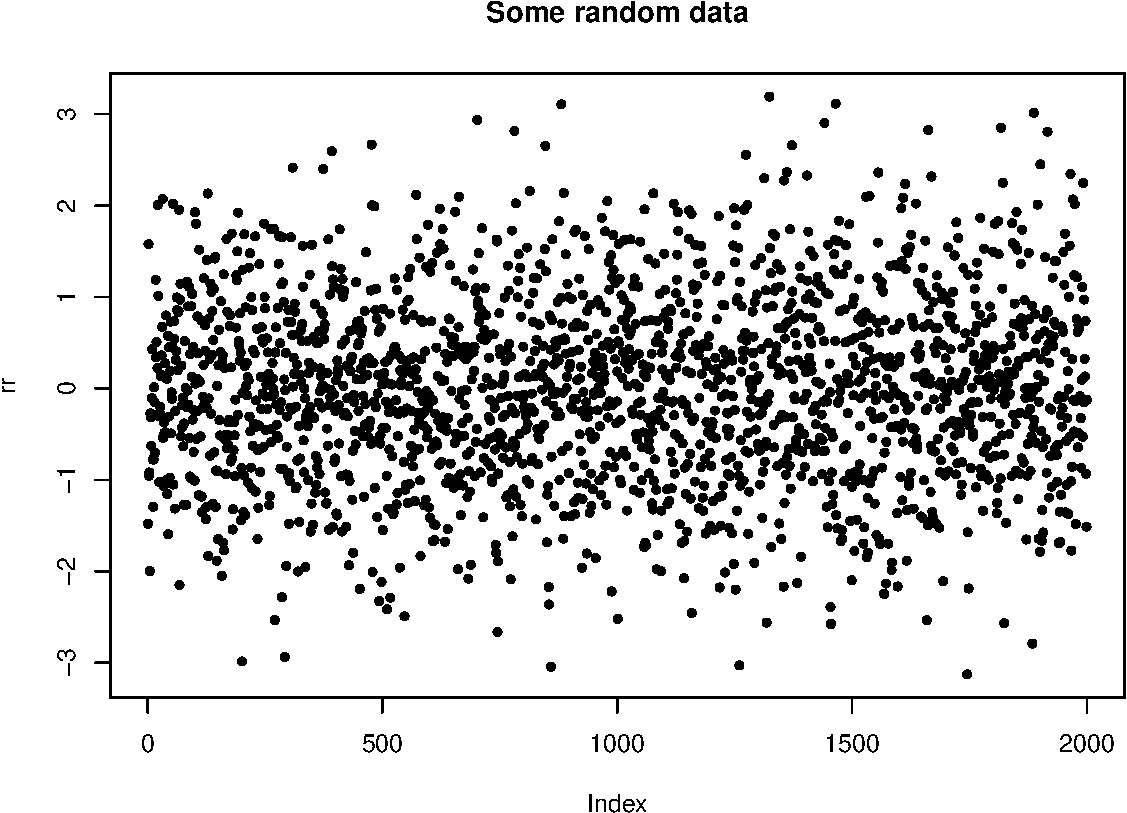
\includegraphics{Lesson5_rmd_files/figure-latex/unnamed-chunk-1-1.pdf}

Figure 1. Example of a stock plot embedded into a PDF from RMarkdown.

\newpage  

\subsection{Show plots with associated
code}\label{show-plots-with-associated-code}

\begin{Shaded}
\begin{Highlighting}[]
\KeywordTok{require}\NormalTok{(viridis)}
\NormalTok{bm <-}\StringTok{ }\DecValTok{0}
\KeywordTok{par}\NormalTok{(}\DataTypeTok{las=}\DecValTok{1}\NormalTok{,}\DataTypeTok{bty=}\StringTok{"n"}\NormalTok{); xlim <-}\StringTok{ }\KeywordTok{c}\NormalTok{(}\OperatorTok{-}\DecValTok{5}\NormalTok{,}\DecValTok{5}\NormalTok{);ylim <-}\StringTok{ }\KeywordTok{c}\NormalTok{(}\DecValTok{0}\NormalTok{,}\FloatTok{0.5}\NormalTok{)}
\KeywordTok{set.seed}\NormalTok{(}\DecValTok{12}\NormalTok{)}
\NormalTok{N <-}\StringTok{ }\DecValTok{2000}
\NormalTok{rr <-}\StringTok{ }\KeywordTok{rnorm}\NormalTok{(N); rr2 <-}\StringTok{ }\KeywordTok{rnorm}\NormalTok{(N}\OperatorTok{^}\DecValTok{2}\NormalTok{); rr3 <-}\StringTok{ }\KeywordTok{rnorm}\NormalTok{(N}\OperatorTok{+}\FloatTok{0.3}\NormalTok{)}
\NormalTok{rrd <-}\StringTok{ }\KeywordTok{density}\NormalTok{(rr);rrd2 <-}\StringTok{ }\KeywordTok{density}\NormalTok{(rr2);rrd3 <-}\StringTok{ }\KeywordTok{density}\NormalTok{(rr3)}
\NormalTok{main <-}\StringTok{ }\KeywordTok{paste0}\NormalTok{(N,}\StringTok{" points but plot better"}\NormalTok{);xlab <-}\StringTok{ "Points in space"}
\ControlFlowTok{if}\NormalTok{(bm}\OperatorTok{==}\DecValTok{1}\NormalTok{)\{}
  \KeywordTok{layout}\NormalTok{(}\KeywordTok{matrix}\NormalTok{(}\KeywordTok{c}\NormalTok{(}\KeywordTok{rep}\NormalTok{(}\DecValTok{1}\NormalTok{,}\DecValTok{3}\NormalTok{),}\DecValTok{2}\OperatorTok{:}\DecValTok{4}\NormalTok{), }\DecValTok{2}\NormalTok{, }\DecValTok{3}\NormalTok{, }\DataTypeTok{byrow =} \OtherTok{TRUE}\NormalTok{));sc <-}\StringTok{ }\DecValTok{1}
  \KeywordTok{plot}\NormalTok{(rr,}\DataTypeTok{las=}\DecValTok{1}\NormalTok{,}\DataTypeTok{bty=}\StringTok{"n"}\NormalTok{,}\DataTypeTok{col=}\KeywordTok{adjustcolor}\NormalTok{(}\KeywordTok{viridis}\NormalTok{(N),}\FloatTok{0.5}\NormalTok{),}\DataTypeTok{pch=}\DecValTok{20}\NormalTok{,}\DataTypeTok{cex=}\KeywordTok{runif}\NormalTok{(}\DecValTok{10}\NormalTok{,}\DecValTok{1}\NormalTok{,}\DecValTok{5}\NormalTok{),}
       \DataTypeTok{main=}\NormalTok{main,}\DataTypeTok{xlab=}\NormalTok{xlab)}
\ControlFlowTok{for}\NormalTok{(r }\ControlFlowTok{in} \KeywordTok{list}\NormalTok{(rrd,rrd2,rrd3))\{}
  \KeywordTok{plot}\NormalTok{(r,}\DataTypeTok{xlim=}\NormalTok{xlim,}\DataTypeTok{ylim=}\NormalTok{ylim,}\DataTypeTok{main=}\StringTok{""}\NormalTok{)}
  \KeywordTok{polygon}\NormalTok{(r,}\DataTypeTok{col=}\KeywordTok{adjustcolor}\NormalTok{(}\KeywordTok{viridis}\NormalTok{(}\DecValTok{250}\NormalTok{)[sc],}\FloatTok{0.5}\NormalTok{),}\DataTypeTok{border=}\KeywordTok{viridis}\NormalTok{(}\DecValTok{250}\NormalTok{)[sc]);sc <-}\StringTok{ }\NormalTok{sc}\OperatorTok{+}\DecValTok{100}\NormalTok{\}}
\NormalTok{\}}\ControlFlowTok{else}\NormalTok{\{}\KeywordTok{par}\NormalTok{(}\DataTypeTok{mfrow=}\KeywordTok{c}\NormalTok{(}\DecValTok{1}\NormalTok{,}\DecValTok{1}\NormalTok{))}
  \KeywordTok{plot}\NormalTok{(rr,}\DataTypeTok{las=}\DecValTok{1}\NormalTok{,}\DataTypeTok{bty=}\StringTok{"n"}\NormalTok{,}\DataTypeTok{col=}\KeywordTok{adjustcolor}\NormalTok{(}\KeywordTok{viridis}\NormalTok{(N),}\FloatTok{0.5}\NormalTok{),}\DataTypeTok{pch=}\DecValTok{20}\NormalTok{,}\DataTypeTok{cex=}\KeywordTok{runif}\NormalTok{(}\DecValTok{10}\NormalTok{,}\DecValTok{1}\NormalTok{,}\DecValTok{5}\NormalTok{),}
       \DataTypeTok{main=}\NormalTok{main,}\DataTypeTok{xlab=}\NormalTok{xlab)\}}
\end{Highlighting}
\end{Shaded}

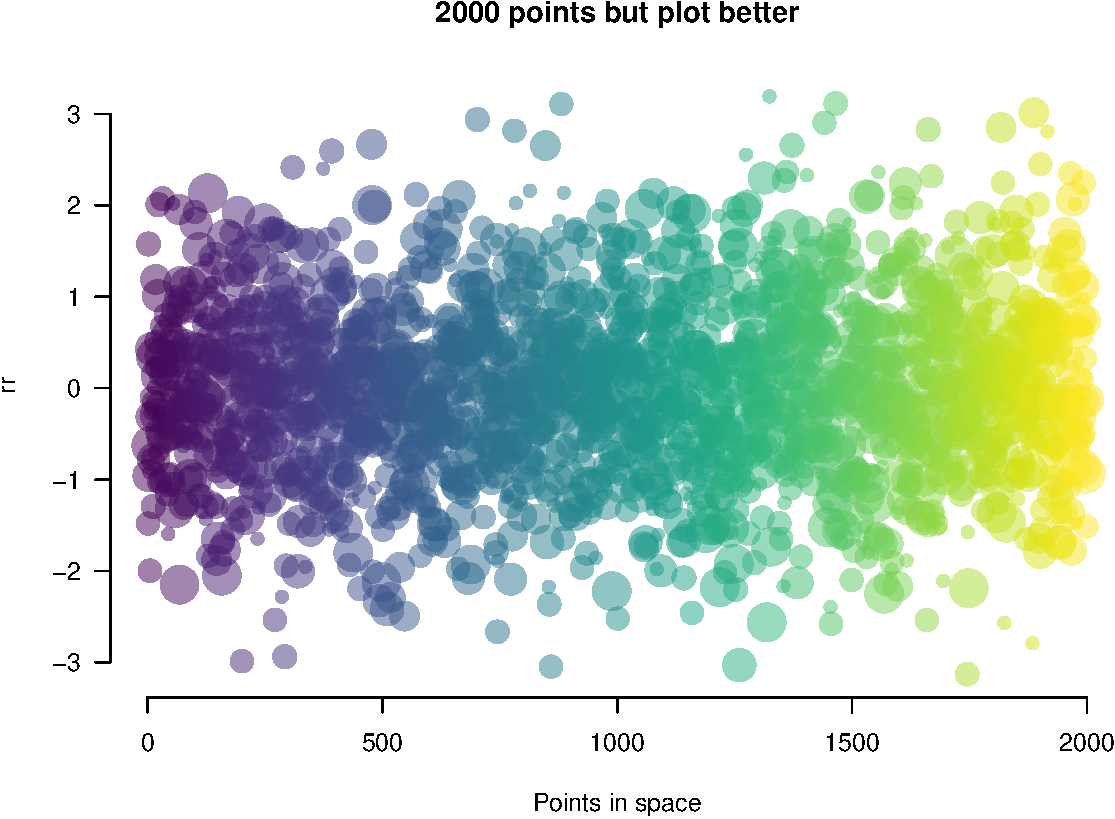
\includegraphics{Lesson5_rmd_files/figure-latex/unnamed-chunk-2-1.pdf}

Figure 2. Example of a plot with improved graphics and its associated
code embedded into a PDF from RMarkdown.

\newpage  

\subsection{And tables}\label{and-tables}

Table 1. Definitions of model parameters for individual hosts and
\textbf{parasites}. Dimensions and units: -, dimensionless; cm,
centimetres; J, Joules; L, length.

\begin{longtable}[]{@{}clr@{}}
\toprule
Parameter & Definition & Dimension(unit)\tabularnewline
\midrule
\endhead
\emph{L} & structural length & cm\tabularnewline
\emph{ee} & scaled reserve density & J
(cm\textsuperscript{3})\tabularnewline
\emph{D} & host development & ---\tabularnewline
\emph{RH} & energy in reproduction buffer & J\tabularnewline
\bottomrule
\end{longtable}

\newpage  

\subsection{Use buttons or tabs for
sub-chapters}\label{use-buttons-or-tabs-for-sub-chapters}

\subsubsection{Chapter 1}\label{chapter-1}

\emph{Then you can add whatever you want here} like you would normally
write in the \texttt{Rmd} file.\\
\hspace*{0.333em}

\subsubsection{Chapter 2 (with new code)}\label{chapter-2-with-new-code}

Here's an Easter egg for you \ldots{}

\begin{verbatim}
## [[1]]
## [1] TRUE
## 
## [[2]]
## [1] TRUE
\end{verbatim}

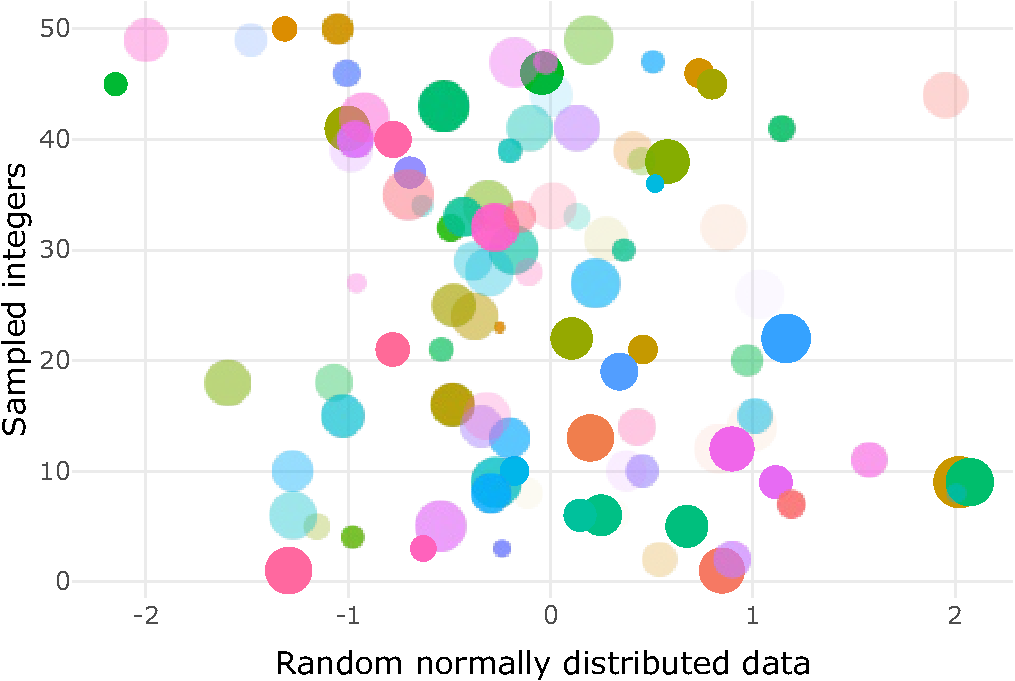
\includegraphics{Lesson5_rmd_files/figure-latex/unnamed-chunk-3-1.pdf}

\subsubsection{More tables}\label{more-tables}

Here's a new way of creating tables using the \texttt{DT} package

\begin{verbatim}
## [[1]]
## [1] TRUE
## 
## [[2]]
## [1] TRUE
\end{verbatim}

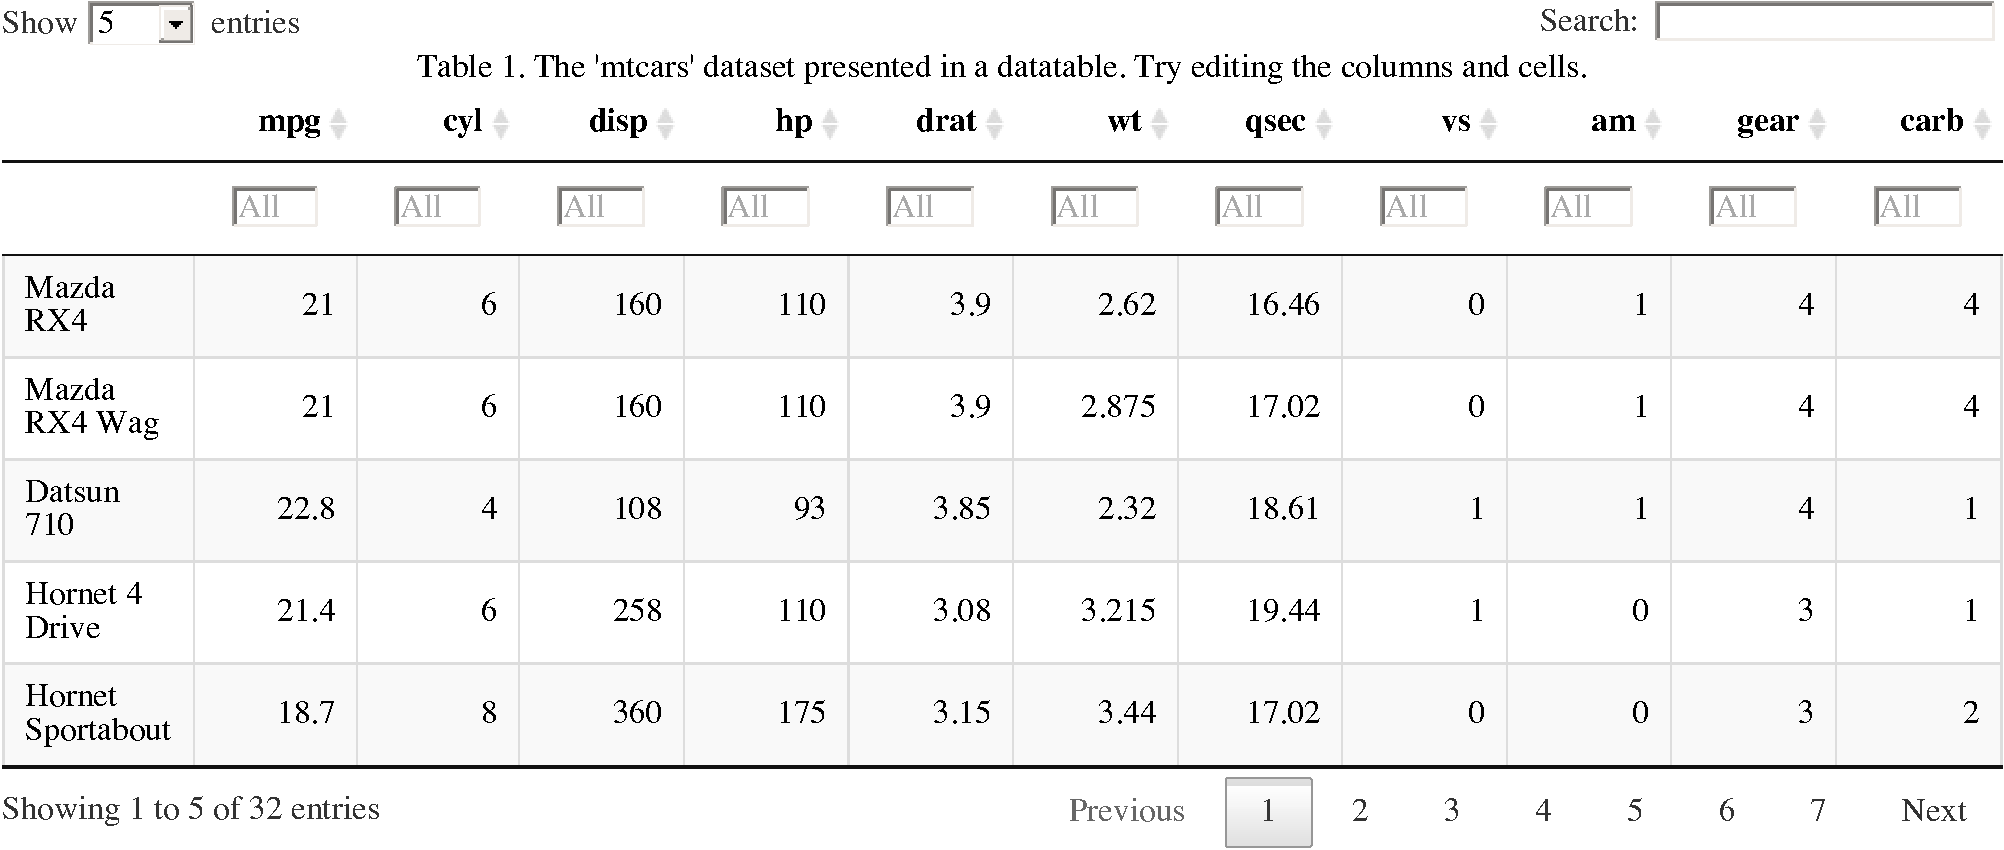
\includegraphics{Lesson5_rmd_files/figure-latex/unnamed-chunk-4-1.pdf}

\begin{center}\rule{0.5\linewidth}{\linethickness}\end{center}

\subsection{Embed code from different
languages}\label{embed-code-from-different-languages}

\subsubsection{\texorpdfstring{This is \texttt{R}
code}{This is R code}}\label{this-is-r-code}

\begin{Shaded}
\begin{Highlighting}[]
\ControlFlowTok{if}\NormalTok{(pck}\OperatorTok{==}\DecValTok{1}\NormalTok{)\{}
\NormalTok{  p<-}\KeywordTok{c}\NormalTok{(}\StringTok{"rJava"}\NormalTok{, }\StringTok{"RNetLogo"}\NormalTok{); }\KeywordTok{remove.packages}\NormalTok{(p)}
  \CommentTok{# then install rJava and RNetLogo from source}
  \KeywordTok{install.packages}\NormalTok{(}\StringTok{"rJava"}\NormalTok{, }\DataTypeTok{repos =} \StringTok{"https://cran.r-project.org/"}\NormalTok{)}
  \KeywordTok{install.packages}\NormalTok{(}\StringTok{"RNetLogo"}\NormalTok{, }\DataTypeTok{repos =} \StringTok{"https://cran.r-project.org/"}\NormalTok{)}
\NormalTok{\}}
\end{Highlighting}
\end{Shaded}

\subsubsection{\texorpdfstring{\texttt{shell/bash}}{shell/bash}}\label{shellbash}

\begin{Shaded}
\begin{Highlighting}[]
\BuiltInTok{echo} \StringTok{"Hello Bash!"}  
\BuiltInTok{pwd} \CommentTok{# check working dir}
\FunctionTok{git}\NormalTok{ init }\CommentTok{# initialise git}
\end{Highlighting}
\end{Shaded}

\subsubsection{\texorpdfstring{Octave (and MATLAB from the
\texttt{RMatlab}
package).}{Octave (and MATLAB from the RMatlab package).}}\label{octave-and-matlab-from-the-rmatlab-package.}

\href{https://cran.r-project.org/web/packages/R.matlab/index.html}{\texttt{RMatlab\ documentation}}.

\begin{Shaded}
\begin{Highlighting}[]
\NormalTok{b = [}\FloatTok{4}\NormalTok{; }\FloatTok{9}\NormalTok{; }\FloatTok{2}\NormalTok{] }\CommentTok{# Column vector}
\NormalTok{A = [ }\FloatTok{3} \FloatTok{4} \FloatTok{5}\NormalTok{;}
      \FloatTok{1} \FloatTok{3} \FloatTok{1}\NormalTok{;}
      \FloatTok{3} \FloatTok{5} \FloatTok{9}\NormalTok{ ]}
\NormalTok{x = A \textbackslash{} b     }\CommentTok{# Solve the system Ax = b}
\end{Highlighting}
\end{Shaded}

\subsubsection{HTML}\label{html}

\begin{Shaded}
\begin{Highlighting}[]
\CommentTok{<!-- links-->}
        \KeywordTok{<div}\OtherTok{ class=}\StringTok{"footer"}\KeywordTok{>}
            \KeywordTok{<a}\OtherTok{ href=}\StringTok{"dd_feed.html"} 
\OtherTok{            class=}\StringTok{"transition fade_in"}\KeywordTok{>}
\NormalTok{                Latest post}
            \KeywordTok{</a>}
            \DecValTok{&nbsp;} \DecValTok{&nbsp;} \DecValTok{&nbsp;}
            \KeywordTok{<a}\OtherTok{ href=}\StringTok{"dd_contact.html"} 
\OtherTok{            class=}\StringTok{"transition fade_in"}\KeywordTok{>}
\NormalTok{                Contact}
            \KeywordTok{</a>}
            \DecValTok{&nbsp;} \DecValTok{&nbsp;} \DecValTok{&nbsp;}
            \KeywordTok{<a}\OtherTok{ href=}\StringTok{"dd_subscribe.html"}
\OtherTok{            class=}\StringTok{"transition fade_in"}\KeywordTok{>}
\NormalTok{                Subscribe}
            \KeywordTok{</a>}
        \KeywordTok{</div>}
\end{Highlighting}
\end{Shaded}

\subsubsection{CSS}\label{css}

\begin{Shaded}
\begin{Highlighting}[]
\NormalTok{# custom code for the tabs in this file}
\FloatTok{.btn} \KeywordTok{\{}
    \KeywordTok{border-width:} \DataTypeTok{0} \DataTypeTok{0px} \DataTypeTok{0px} \DataTypeTok{0px}\KeywordTok{;}
    \KeywordTok{font-weight:} \DataTypeTok{normal}\KeywordTok{;}
    \KeywordTok{text-transform:} \KeywordTok{;}
\KeywordTok{\}}
\FloatTok{.btn-default} \KeywordTok{\{}
    \KeywordTok{color:} \DataTypeTok{#f08080}\KeywordTok{;}
    \KeywordTok{background-color:} \DataTypeTok{#ffffff}\KeywordTok{;}
    \KeywordTok{border-color:} \DataTypeTok{#ffffff}\KeywordTok{;}
\KeywordTok{\}}
\end{Highlighting}
\end{Shaded}

\subsubsection{\texorpdfstring{Javascript to access \texttt{html} and
\texttt{css}}{Javascript to access html and css}}\label{javascript-to-access-html-and-css}

\begin{Shaded}
\begin{Highlighting}[]
\AttributeTok{$}\NormalTok{(}\StringTok{'.title'}\NormalTok{).}\AttributeTok{css}\NormalTok{(}\StringTok{'color'}\OperatorTok{,} \StringTok{'red'}\NormalTok{)}
\end{Highlighting}
\end{Shaded}

\subsubsection{Python}\label{python}

\begin{Shaded}
\begin{Highlighting}[]
\NormalTok{x }\OperatorTok{=} \StringTok{'hello, python world!'}
\BuiltInTok{print}\NormalTok{(x.split(}\StringTok{' '}\NormalTok{))}
\end{Highlighting}
\end{Shaded}

\subsubsection{Here's a complete list of available
languages}\label{heres-a-complete-list-of-available-languages}

\begin{Shaded}
\begin{Highlighting}[]
\KeywordTok{names}\NormalTok{(knitr}\OperatorTok{::}\NormalTok{knit_engines}\OperatorTok{$}\KeywordTok{get}\NormalTok{())}
\end{Highlighting}
\end{Shaded}

\begin{verbatim}
##  [1] "awk"       "bash"      "coffee"    "gawk"      "groovy"   
##  [6] "haskell"   "lein"      "mysql"     "node"      "octave"   
## [11] "perl"      "psql"      "Rscript"   "ruby"      "sas"      
## [16] "scala"     "sed"       "sh"        "stata"     "zsh"      
## [21] "highlight" "Rcpp"      "tikz"      "dot"       "c"        
## [26] "fortran"   "fortran95" "asy"       "cat"       "asis"     
## [31] "stan"      "block"     "block2"    "js"        "css"      
## [36] "sql"       "go"        "python"    "julia"     "sass"     
## [41] "scss"
\end{verbatim}

\end{document}
